\PassOptionsToPackage{brazil,american}{babel}
\documentclass[12pt]{article}

\usepackage{sbc-template}
\usepackage[brazil,american]{babel}
\usepackage[utf8]{inputenc}

\usepackage{graphicx}
\usepackage{url}
\usepackage{float}
\usepackage{listings}	
\usepackage{color}
\usepackage{todonotes}
\usepackage{algorithmic}
\usepackage{algorithm}
\usepackage{hyperref}

\sloppy

\title{Experimento 8\\ 
	FLIP-FLOPS:RS E JK}

\author{
	Lucas Mafra Chagas, 12/0126443 \\
	Marcelo Giordano Martins Costa de Oliveira,  12/0037301
}


\address{Dep. Ciência da Computação -- Universidade de Brasília (UnB)\\
	CiC 116351 - Circuistos Digitais - Turma C
	\email{\{giordano.marcelo, chagas.lucas.mafra\}@gmail.com}
}

\begin{document} 

\maketitle

 \begin{abstract}
	 In this experiment, we will study some types of flip-flops RS and JK by implementing, verifying their truth tables and comparing with the theoretical well-known results.
 \end{abstract}
     
 \begin{resumo} 
	 Neste experimento, serão estudados os alguns tipos de flip-flops RS e JK, através de sua implementação e posterior verificação de suas respectivas tabelas verdade, comparando-as com os resultados esperados teoricamente.
 \end{resumo}


\section{Objetivos}
\label{sec:Objetivos}

Apresentação do flip-flop como unidade armazenadora de memória. Observação do funcionamento e construção dos flip-flops RS, RS Gatilhado, SENHOR-ESCRAVO e JK SENHOR-ESCRAVO.

\section{Materiais} 
\label{sec:Materiais}

\begin{itemize}
    \item Painel Digital
    
    \item \textit{protoboard}
    
    \item Fios
    
    \item Portas Lógicas NAND, NOR e NOT.
    
\end{itemize}


\section{Introdução}
\label{sec:Introducao}

O flip-flop, ou multivibrador biestável, é um circuito digital pulsado capaz de servir como uma memória de um bit. Um flip-flop tipicamente tem dois sinais de entrada, o \textit{SET} e o \textit{RESET}, um sinal de clock (gatilho), um sinal de saída e o seu inverso. A pulsação ou mudança no sinal do clock faz com que o flip-flop mude ou retenha seu sinal de saída, baseado nos valores dos sinais de entrada e na equação característica do flip-flop. Existem vários tipos de flip-flops.

\subsection{Flip-flop Latch RS}
O valor guardado no flip-flop será mantido se \textit{SET} e \textit{RESET} forem ambos iguais a 0; irá mudar para 0, se a entrada \textit{RESET} for 1, e se tornará 1 se a entrada \textit{SET} for 1. O comportamento não será especificado se as duas entradas forem iguais a 1. Esse comportamento, neste relatório será referido como o estado proibido. Aqui temos uma implementação desse flip-flop feito apenas com portas NAND.

\begin{figure}[H]
	\centering
	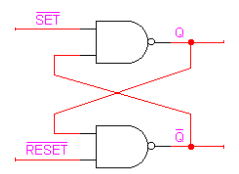
\includegraphics[width=.5\textwidth]{latchRS.png}
	\caption{Latch RS}
	\label{fig:latRS}
\end{figure}

Para este tipo de implementação temos que considerar que a ativação de \textit{SET} ou \textit{RESET} é feita quando a entrada é 0. Além disso, temos que para esse flip-flop a saída possui um complemento, que sempre será o inverso da saída original.

\subsection{Flip-Flop RS Gatilhado}

Aqui há a inclusão de um gatilho(toggle) T. Quando houver variação do clock, o valor guardado no flip-flop será alternado ou mantido dependendo se o valor na entrada T (gatilho), se ele está em 1 ou 0. Se o valor de T é 1 temos que o valor será alterado de acordo com as entradas em \textit{SET} e \textit{RESET}. Se o valor de T é 0, o último valor alterado será armazenado, pois \textit{$\overline{SET}$} e \textit{$\overline{RESET}$} serão ambos iguais a 0. Portanto, a cada pulso de T temos o armazenamento da última mudança feita no flip-flop.

\begin{figure}[H]
	\centering
	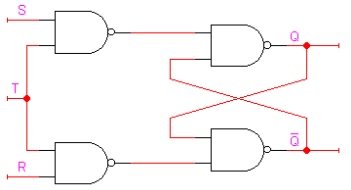
\includegraphics[width=.5\textwidth]{RSgat.png}
	\caption{Latch RS Gatilhado}
	\label{fig:RSgat}
\end{figure}

Para este flip-flop temos também a entrada proibida. Se ambos o \textit{SET} e o \textit{RESET} estiverem ativados, a saída será indeterminada.


\subsection{Flip-Flop RS Gatilhado com PRESET e CLEAR}

Este flip-flop é um Flip-Flop RS Gatilhado mas que pode forçar um resultado desejado na saída Q, já que as entradas \textit{RESET} e \textit{CLEAR} funcionam independentemente do gatilho T e das entradas \textit{SET} e \textit{RESET}.

\begin{figure}[H]
	\centering
	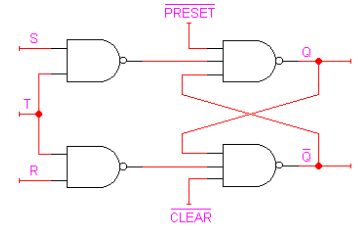
\includegraphics[width=.5\textwidth]{RSgatPC.png}
	\caption{Latch RS Gatilhado com PRESET e CLEAR}
	\label{fig:RSgatPC}
\end{figure}

\subsection{Flip-Flop SENHOR-ESCRAVO}

Este flip-flop é a junção de dois flip-flops RS Gatilhados. As saídas do primeiro flip-flop são as entradas do segundo. O gatilho T porém, nunca possui o mesmo valor nos diferentes flip-flops. Se o gatilho é 1 no flip-flop SENHOR, temos que os valores neste flip-flop podem ser alterados mas o flip-flop ESCRAVO, que terá seu gatilho em 0 permanecerá em repouso. Quando desligamos o gatilho do flip-flop SENHOR, acionamos o escravo, que pegará a informação armazenada no senhor e a armazenará também. Portanto, a cada pulso do gatilho temos que o valor no flip-flop SENHOR será alterado e essa alteração será transferida para o ESCRAVO.

\begin{figure}[H]
	\centering
	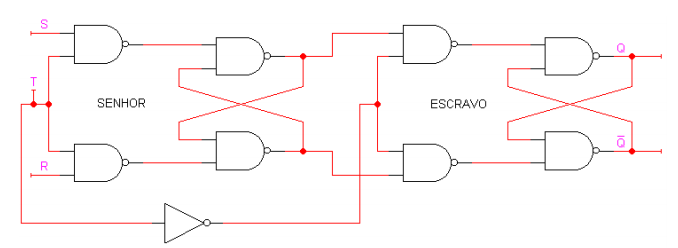
\includegraphics[width=.5\textwidth]{ffMS.png}
	\caption{Flip-Flop SENHOR-ESCRAVO (Master-Slave)}
	\label{fig:ffMS}
\end{figure} 

\subsection{Flip-Flop JK SENHOR-ESCRAVO}

Este flip-flop permite a utilização do antes estado proibido. Temos que quando houver variação do clock, o valor guardado no flip-flop será alternado se as entradas J e K forem ambas iguais a 1 e será mantido se ambas forem iguais a zero. Se forem diferentes, haverá o \textit{SET} ou o \textit{RESET} dos valores.

\begin{figure}[H]
	\centering
	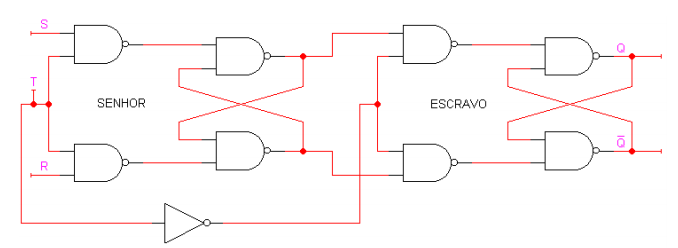
\includegraphics[width=.5\textwidth]{ffJKMS.png}
	\caption{Flip-Flop JK SENHOR-ESCRAVO (Master-Slave)}
	\label{fig:ffJKMS}
\end{figure} 

\section{Procedimentos}
\label{sec:Procedimentos}

Escreva nesta seção os diversos itens pedidos no experimentos. 


\section{Análise dos Resultados}
\label{sec:Resultados}

Faça uma análise crítica dos resultados obtidos nos experimentos. Esta análise pode ser feita item a item ou de uma forma geral.

Dica: Use pesquisa na Internet para tirar as dúvidas sobre edição em \LaTeX .

\section{Conclusão}
\label{sec:Conclusao}

Neste experimento foi possível perceber a importância de um flip-flop na utilização de armazenamento de informações. Vimos que, se construídos corretamente, os flip-flops podem ser úteis em diversas aplicações

\newpage 
% Colocar aqui apenas as respostas dos itens da Auto-Avaliação
\section*{Auto-Avaliação}

\begin{enumerate}
    \item d
    \item a
    \item d
    \item d
    \item c
    \item a
    \item a
\end{enumerate}


\end{document}
